\documentclass{ali-presentation}

\usepackage{fontspec}

\usepackage{minted}
\setminted{
    autogobble,
    frame=topline,
    framesep=10pt,
}

\usepackage{graphicx}

\hypersetup{
  colorlinks=true,
  allcolors=.,
  urlcolor=magenta,
}

\title{Python and Polars}
\subtitle{Predoc Orientation 2025}

\date{July 28, 2025}
\author{Alistair Pattison}

\begin{document}

\maketitle

\begin{frame}[t]
    \frametitle{Python}

    Python is a very popular, very general-purpose programming language

    \pause \centering \bigskip

    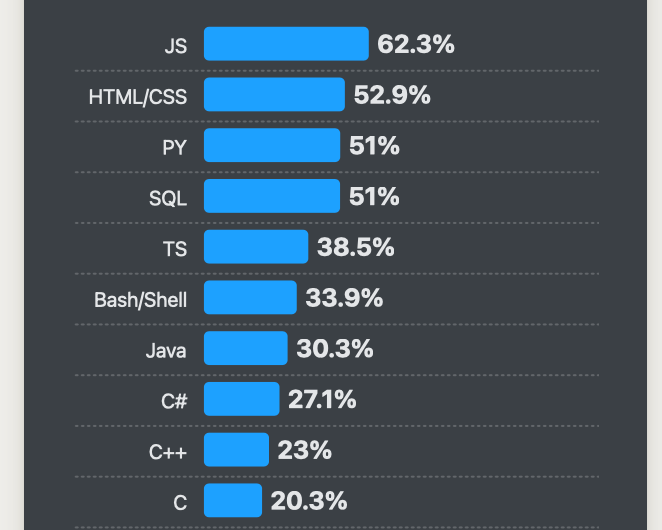
\includegraphics[width = .4 \textwidth]{figures/so-rank.png}
    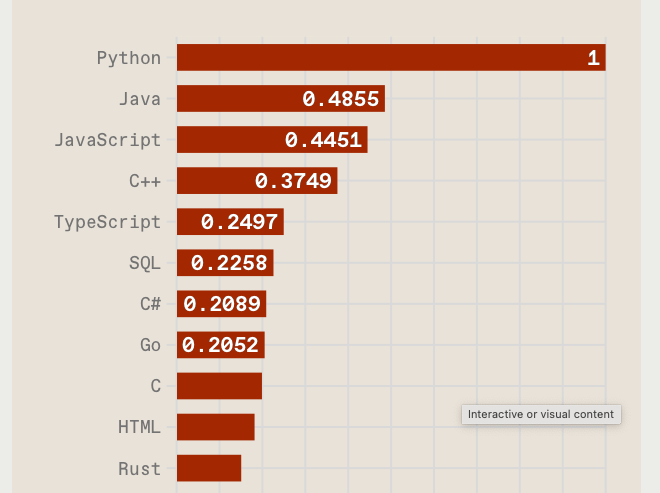
\includegraphics[width = .4 \textwidth]{figures/ieee-rank.png}
\end{frame}

\begin{frame}[t]
    \frametitle{Polars}

    Polars is a DataFrame library for Python. It's like Pandas but
    \begin{itemize}
        \item \href{https://pola.rs/posts/benchmarks/}{literally 25-100x faster}
        \item with a much, much, nicer API
    \end{itemize}

    \pause \centering

    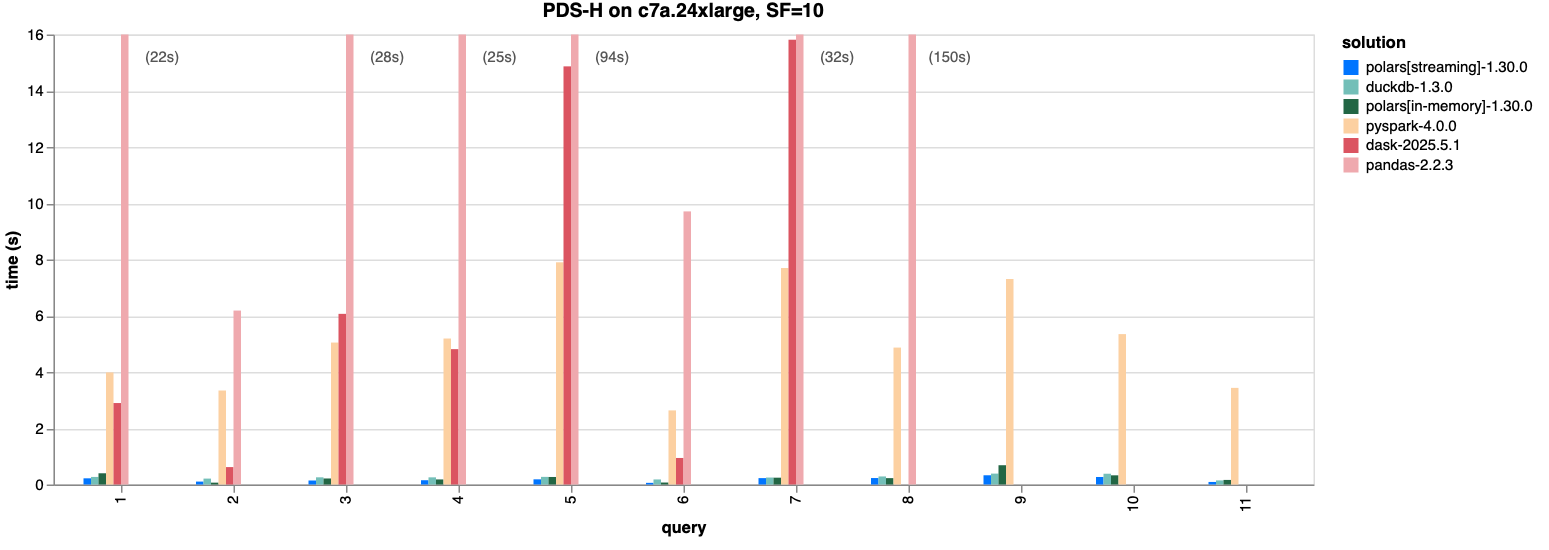
\includegraphics[width = \textwidth]{figures/benchmarks.png}
\end{frame}

\begin{frame}[b]
    \centering
    
\includegraphics[height = .9\textheight]{figures/handshake.jpg}
\end{frame}

\begin{frame}
    \frametitle{Today}

    \tableofcontents
\end{frame}

% different ways to run python scripts
% interactively in the terminal
% as a script

\section{Python 101}

\begin{frame}
    \frametitle{Step 0}

    \begin{itemize}
        \item Install python
            (I recommend using \href{https://docs.astral.sh/uv/getting-started/installation/}{\texttt{uv}})
            \begin{itemize}
                \item \texttt{curl -LsSf https://astral.sh/uv/install.sh | sh}
                \item \texttt{uv python install --preview --default}
            \end{itemize}
        \item Create and activate a virtual envrionment
            \begin{itemize}
                \item \texttt{mkdir python-practice \&\& cd python-practice}
                \item \texttt{uv venv \&\& source .venv/bin/activate}
            \end{itemize}
        \item Make sure everything works
            \begin{itemize}
                \item \texttt{python -c "import sys; print('hello from python', sys.version)"}
                \item Should output something like \texttt{"hello from python 3.13.1 ..."}
            \end{itemize}
    \end{itemize}
\end{frame}

\begin{frame}[fragile]
    \frametitle{A Very Simple Python Script}

    \begin{minted}[label=example.py]{python}
        def main(x): # define a function
            y = x * 2
            for i in range(y):
                print("hello world!", i)

        main(3) # will print "hello world! 0", "hello world! 1", ...
    \end{minted}
    
    To run this script you can
    \begin{itemize}
        \item Open a python terminal (\texttt{python}), paste this, and press enter
        \item Run via the command line: \texttt{python example.py}
        \item Use a \href{https://jupyter.org}{jupyter notebook}
    \end{itemize}
\end{frame}

\begin{frame}[fragile,t]
    \frametitle{Modules and Imports}

    \begin{columns}[t]
        \begin{column}{.5\textwidth}
            \begin{minted}[label=complicated.py]{python}
                from math import sqrt, exp

                def foo(x):
                    return exp(1 / sqrt(3 * x))
            \end{minted}
        \end{column}
        \pause
        \begin{column}{.5\textwidth}
            \begin{minted}[label=main.py]{python}
                import complicated
                
                print(complicated.foo(100)) 
            \end{minted}
        \end{column}
    \end{columns}

    \bigskip
    \pause
    
    Put both files in the same folder and run with the \texttt{-m} flag and no \texttt{.py} suffix:

    \begin{minted}[frame=none]{text}
        $ python -m main
        1.05943423696
    \end{minted}

    \pause

    Can have more complicated/nested imports. See e.g. \href{https://medium.com/@officialyrohanrokade/mastering-python-imports-and-module-management-a-deep-dive-into-import-keywords-folder-d92aa1daaaf5}{this article}.
\end{frame}

\begin{frame}[fragile, t]
    \frametitle{Type Hints}

    \begin{columns}[t]
        \begin{column}{.5\textwidth}
            \begin{minted}[label=complicated.py, highlightlines=3]{python}
                from math import sqrt, exp

                def foo(x):
                    return exp(1 / sqrt(3 * x))
            \end{minted}
        \end{column}
        \pause
        \begin{column}{.5\textwidth}
            \begin{minted}[label=complicated.py, highlightlines=3]{python}
                from math import sqrt, exp

                def foo(x: int | float) -> float:
                    return exp(1 / sqrt(3 * x))
            \end{minted}
        \end{column}
    \end{columns}

    \pause \bigskip

    \begin{minted}[label=main.py]{python}
        import complicated
        
        print(complicated.foo(100)) # <- all good!
        print(complicated.foo("cat")) # <- editor will give you a
                                      #    squiggly red underline
    \end{minted}
\end{frame}

\begin{frame}
    \frametitle{Packages}

    \begin{itemize}
        \item Python ships with an enormous ``standard library'' (built-in functions)
            \begin{itemize}
                \item Examples: \texttt{datetime}, \texttt{tempfile} (temporary files), \texttt{pathlib} (paths), \texttt{gzip} (compression), \texttt{threading} (parallelization), \texttt{email}, \texttt{re} (regular expressions)
                \item \href{https://docs.python.org/3/library/index.html}{Documentation}
            \end{itemize}
        \item Users can write their own packages and publish them on \href{https://pypi.org}{PyPi}
            \begin{itemize}
                \item Examples: \texttt{requests}/\texttt{beautifulsoup} (web requests), \texttt{flask}/\texttt{django} (web sites), \texttt{typer} (command line apps), \texttt{ipython}/\texttt{jupyter} (different ways to run python)
            \end{itemize}
        \item Other users can install them with the python package manager \texttt{pip}
            \begin{itemize}
                \item E.g., \texttt{pip install polars}
            \end{itemize}
    \end{itemize}
\end{frame}

\section{Polars 101}

\setminted{frame=none}

\begin{frame}
    \frametitle{Polars is...}

    \begin{itemize}
        \item A dataframe library for Python
        \item Easy to use
            \begin{itemize}
                \item Has a tidyverse-esque API
                \item Syntax is succinct and easy to read
            \end{itemize}
        \item Able to do a lot
            \begin{itemize}
                \item String manipulations, datetimes, window expressions, etc.
                \item Exendable via plug-ins: OLS, shrinkage, weighted means, etc.
            \end{itemize}
        \item Lazy 
            \begin{itemize}
                \item More on next slide
            \end{itemize}
    \end{itemize}
\end{frame}


\begin{frame}[fragile]
    \frametitle{Minimal Example}

    \begin{minted}{python}
        import polars as pl

        # construct (but don't execute) query
        query = (
            pl.scan_csv("databank.parquet") 
            .filter(pl.col("year").is_between(2010, 2020))
            .group_by("year", "sex", "age")
            .agg(
                pl.col("died").mean().alias("mr"), # <- "expressions"
                pl.len().alias("population"),
            )
        )

        print(query.collect()) # now execute the query
    \end{minted}
\end{frame}


\begin{frame}
    \frametitle{Lazy Evaluation}

    Polars gets a lot of its speed from being \textit{lazy}:

    \begin{itemize}
        \item Doesn't load data up-front (e.g. \texttt{pl.scan\_csv(...)})
        \item Processes the whole query at once when you call \texttt{.collect()}
    \end{itemize}

    \pause

    This has many benefits:

    \begin{itemize}
        \item Runs every step all at once and in parallel (huge speed boost)
        \item Can optimize query (e.g. to cache reused portions)
        \item Loads only the data required for a particular query (lower memory use)
        \item Can process datasets that don't fit into memory (more later)
    \end{itemize}
\end{frame}

\begin{frame}
    \frametitle{Aside: About Documentation}

    \begin{itemize}
        \item Please read documentation 
            \begin{itemize}
                \item
                    \href{https://docs.pola.rs/api/python/stable/reference/index.html}{Polars};
                    \href{https://docs.python.org/3/library/index.html}{Python standard library}
            \end{itemize}
        \item Docs help you learn features you would not know exist otherwise
        \item ChatGPT is great for ``how do i do xyz?"
        \item ... but still read the damn documentation 
    \end{itemize}
    
\end{frame}

\section{Cookbook}

\begin{frame}[fragile]
    \frametitle{Paths / Project Root}

    \begin{minted}{python}
        from pathlib import Path # <- part of the standard library
        from git import Repo # <- pip install gitpython

        _REPO = Repo('.', search_parent_directories=True)

        PROJECT_ROOT = Path(_REPO.working_tree_dir)

        DATA = PROJECT_ROOT / "data" # path relative to root
    \end{minted}
\end{frame}

\begin{frame}[fragile]
    \frametitle{Loading Data}

    \begin{minted}{python}
        import polars as pl
        import polars_io as pio # <- written by yours truly :D
        from paths import DATA

        pl.scan_parquet(DATA / "new_databank.parquet") # parquet

        pio.scan_sas7bdat(DATA / "sas_file.sas7bdat") # sas
        pio.scan_dta("stata_file.dta") # stata
        pio.scan_fwf( # fixed-width file
            "fixed_width.txt",
            { "county" : (0, 3), "population", (7, 14) } # col locations
        )
    \end{minted}
\end{frame}

\begin{frame}[fragile]
    \frametitle{Joins}

    \begin{minted}{python}
            db = pl.scan_csv("databank.parquet")
            county_attrs = pl.scan_csv("county_level_attributes.parquet")

            db.join(
                county_attrs,
                on = ["year", "state", "county"],
                how = "left",
                validate = "m:1", # will throw error if not met
            )
    \end{minted}
\end{frame}


\begin{frame}
    \frametitle{Auto-formatting / Linting / Type-checking}
    
    \begin{itemize}
        \item Formatters and linters make your life so much easier!
        \item In VSCode: search \texttt{ruff}. (I recommend turning on ``format on save".)
        \item From the command line: (works on the inside!): \texttt{pip install ruff}, \texttt{ruff check --fix}, \texttt{ruff format}.
    \end{itemize}
\end{frame}

\begin{frame}[fragile]
    \frametitle{Figures}

    \begin{minted}{python}
        # see also matplotlib.org for an alternative
        import plotnine as pn # plotnine.org
        from plotnine.data import anscombe_quartet 

        plots = [
            pn.ggplot(anscombe_quartet, pn.aes("x", "y", color="dataset"))
            + pn.geom_point(),
            pn.ggplot(anscombe_quartet, pn.aes("x", "y", color="dataset"))
            + pn.geom_point()
            + pn.facet_wrap("dataset")
        ]

        save_as_pdf_pages(plots, "~/Downloads/plots.pdf")
    \end{minted}
\end{frame}

\begin{frame}[fragile]
    \frametitle{Tables}

    \begin{minted}{python}
        # posit-dev.github.io/great-tables/examples/
        from great_tables import GT

        ...

        (
            GT(wide_pops)
            .tab_header(title="Populations of Oceania's Countries")
            # add header above certain columns
            .tab_spanner(label="Total Population", columns=cs.all())
            # add sections based on columns
            .tab_stub(rowname_col="country_name", groupname_col="region")
            .fmt_integer()
            .as_latex() # <- output as latex
        )
    \end{minted}
\end{frame}

\begin{frame}[fragile]
    \frametitle{Repeating Common Functionality}

    \begin{minted}{python}
        def calculate_mortality_rate(
            df: pl.LazyFrame,
            col_name="mortality_rate"
        ) -> pl.LazyFrame:
            df.with_columns(
                pl.when(pl.col("population") > 0)
                .then(pl.col("deaths") / pl.col("population"))
                .otherwise(None)
                .alias(col_name)
            ) 

        # call df.pipe to use the function in a pipeline
        mortality = deaths_and_pops.pipe(calculate_mortality_rate, "mr")
    \end{minted}
\end{frame}

\begin{frame}[fragile]
    \frametitle{Larger-than-memory data}

    \begin{minted}{python}
        # describe plan
        plan = (
            pl.scan_csv("heinous_200_gb_csv.csv")
            .with_columns(age = pl.col("birth_date") - pl.col("year"))
        )

        # "sink" to a file
        plan.sink_csv("processed_data.csv", engine="streaming")
        # or even better:
        # .sink_parquet("processed_data.parquet", engine="streaming"))
    \end{minted}
\end{frame}

\begin{frame}[fragile]
    \frametitle{Window Expressions}

    \begin{minted}{python}

        demeaned_inc = (
            pl.col("inc_rank")
            - pl.col("inc_rank").mean().over("year", "county")
        )

        last_years_inc = (
            pl.col("inc_rank")
            .shift(1)
            .over("pik", order_by = "year")
        )

        # super duper fast!! all groups can run in parallel!!
        df.with_columns(demeaned_inc, last_years_inc)
    \end{minted}
\end{frame}

\begin{frame}[fragile]
    \frametitle{Regressions}

    \begin{minted}{python}
        import polars_ols as pls # github.com/azmyrajab/polars_ols
        from polars import selectors as cs

        df.with_columns(
            pl.col("y") # regress y on...
            .pipe(
                pls.compute_least_squares,
                cs.starts_with("x_"), # every column that starts with x_
                add_intercept=True,
                sample_weight="population",
            )
            .over("year") # regress separately within each year
        )

        # this package can also do l1/2 penalties!
    \end{minted}
\end{frame}

\begin{frame}[fragile]
    \frametitle{Weighted Means, Variances, etc.}

    \begin{minted}{python}
        import polars_utils.stats import mean, var, cov, cor

        df.with_columns(
            pl.col("x").pipe(mean, w = "population"), # mean
            pl.col("x").pipe(var, w = "population"), # var
            pl.col("x").pipe(cov, "y", w = "population"), # cov
            pl.col("x").pipe(cor, "y", w = "population"), # (pearson) cor
        )
    \end{minted}
\end{frame}

\begin{frame}[fragile]
    \frametitle{Shrinkage}

    \begin{minted}{python}
        import polars_utils.shrinkage import * # <- star means "everything"

        # df is a data frame with a column of estimates `beta`
        # and their variances `beta_var`

        df.with_columns(
            rho=pl.col("beta").pipe(reliability, variances="beta_var"),
            beta_shrunk=pl.col("beta").pipe(shrink, variances="beta_var"),
        )
    \end{minted}
\end{frame}

\begin{frame}[fragile]
    \frametitle{Caching}

    \begin{minted}{python}
        # pip install git+https://github.com/alipatti/polars_cache.git
        import polars_cache import cache_to_disc 
        import time
        
        def cached_expensive_function(x: int, y: "abc"):
            return (
                pl.select(x=x + pl.int_range(100), y=y)
                # ... imagine more slow stuff here
                .pipe(cache_to_disc, max_age = 120) # in seconds
            )
            
        expensive_function(10, "abc").collect() # will take a long time
        expensive_function(10, "abc").collect() # fast -- will load from cache
        expensive_function(12, "xyz").collect() # slow because diff args
    \end{minted}

\end{frame}

\begin{frame}[fragile]
    \frametitle{Getting Census Tables}

    \begin{minted}{python}
        import tidycensus
        
        api = Census()
        
        # returns polars df with columns
        # ["year", "county", "concept", "label", "variable", "value"]
        api.get_variables(
            "acs/acs5",
            years=[2010, 2019],
            variables=["B19013_001E", "B19013A_001E"],
            geography="county",
        )
    \end{minted}
\end{frame}

\begin{frame}[fragile]
    \frametitle{Web Scraping}

    \begin{minted}{python}
        import requests
        import parsel
        # ^ I prefer this library but beautiful soup is more popular
        # (https://www.crummy.com/software/BeautifulSoup/bs4/doc/)

        url = "https://opportunityinsights.org/team"
        with requests.get(url) as r:
            s = parsel.Selector(text = r.text)

        names = s.css(".team-member .name ::text").getall()
        # ['Gregory Bruich', 'Stefanie DeLuca', ..., 'Austin Zheng']
    \end{minted}
\end{frame}


\end{document}
